%\motto{Use the template \emph{chapter.tex} to style the various elements of your chapter content.}
\chapter{Quanteninformationen}
\label{qbits} % Always give a unique label
% use \chaptermark{}
% to alter or adjust the chapter heading in the running head

\chapterauthor{Burak Demirtas, Dominik Neumaier, Hannes Ringswald, Marvin Rothmann, Thilo Prünte}

\abstract{}
Dieses Kapitel führt in die Grundlagen der Quanteninformation ein und beschreibt den fundamentalen Unterschied zwischen klassischen Bits und Qubits. Es erklärt die Superposition von Qubits, deren Darstellung auf der Bloch-Kugel sowie die mathematische Dirac-Notation zur effizienten Formulierung quantenmechanischer Zustände und Operatoren. Anschließend werden wesentliche Quanten-Gatter wie die Pauli- und Hadamard-Gatter vorgestellt, die Transformationen von Qubit-Zuständen ermöglichen und Grundlage für Quantenalgorithmen sind. Das Kapitel beschreibt erste Quantenalgorithmen, darunter den Deutsch- und Deutsch-Josza-Algorithmus, die die Effizienzvorteile quantenmechanischer Berechnungen demonstrieren. Weiterhin werden Konzepte der Quantenverschränkung und Quantenteleportation erläutert, inklusive deren Protokolle, Anwendungen in der Quantenkommunikation sowie ihre Realisierung auf Basis von Bell-Zuständen. Abschließend wird die Bedeutung der Bell-Zustände als Basis maximaler Verschränkung und ihre Nutzung in Quantencomputing, Kryptographie und Netzwerken behandelt. Das Kapitel bietet somit einen umfassenden Überblick über zentrale theoretische und praktische Prinzipien der Quanteninformation als Grundlage für weiterführende Quantencomputeranwendungen.

\section{Der Qubit als Informationsträger}
\subsection{Klassisches Bit vs.\ Qubit}
Ein \emph{Bit} ist die kleinste Informationseinheit in klassischen Computern. Es kann genau einen von zwei Zuständen annehmen:
\[
\text{Bit}\,\in\{0,1\}.
\]
Physikalisch bedeutet das zum Beispiel: Strom an = 1, Strom aus = 0. Durch Schaltkreise, die verschiedene logische Operatoren abbilden, können so Berechnungen durchgeführt werden oder durch spezielle Kodierungen (zum Beispiel Ascii) Daten repräsentiert werden.

Ein \emph{Qubit} ist das Gegenstück im \emph{Quantencomputer}. Zunächst wird ein Qubit hier als abstraktes mathematisches Objekt betrachtet. Im späteren Teil dieses Buches wird ein Qubit durchaus auch als konkretes physikalisches Objekt betrachtet, an dieser Stelle soll aber das abstrakte Konzept beschrieben werden, welches auf alle konkreten Umsetzungen zutrifft. 

Wie ein klassisches Bit hat auch auch ein Qubit zwei mögliche Zustände: $\ket{0}$ und $\ket{1}$. Diese Zustände können analog zu $0$ und $1$ in einem klassischen Bit gesehen werden. Die Notation, die zur Beschreibung verwendet wird, heißt \emph{Dirac-Notation} (vgl. Kabitel \ref{subsec:dirac}). Der entscheidende Unterschied zu einem konventionellen Bit ist, dass ein Qubit auch andere Zustände als $\ket{0}$ und $\ket{1}$ annehmen kann. Konkret kann eine lineare Kombination der beiden Zustände, eine sogenannte Superposition (vgl. Kapitel irgendwas in physikalische Grundlagen), einnehmen kann. Dies wird so beschrieben: 
\begin{equation}
    \ket{\psi} = \alpha\,\ket{0} \;+\; \beta\,\ket{1}, \quad \alpha, \beta \in \mathbb{C},
\end{equation}

wobei für \(\alpha\) und \(\beta\) gilt, dass

\begin{equation}
\label{equ:propa}
|\alpha|^2 + |\beta|^2 = 1.
\end{equation}

Die Werte \(|\alpha|^2\) und \(|\beta|^2\) sind die Wahrscheinlichkeiten, das Qubit bei einer Messung in Zustand \(\ket{0}\) bzw.\ \(\ket{1}\) zu finden. In dieser Tatsache erklärt sich auch Formel \ref{equ:propa}: Die Wahrscheinlichkeit, dass das Qubit bei einer Messung einen der beiden Zustände annimmt ist immer 1. 

Als Beispiel soll hier folgender Qubit Zustand dienen, welcher im Verlauf des Buches häufiger als Beispiel verwendet wird:

\begin{equation}
\label{equ:basicZustand}
    \frac{1}{\sqrt{2}}\ket{0} + \frac{1}{\sqrt{2}}\ket{1}
\end{equation}

Um zu überprüfen, ob dies ein gültiger Qubit Zustand ist, werden die Werte in Formel \ref{equ:propa} eingesetzt:

\begin{equation}
    |\frac{1}{\sqrt{2}}|^2 + |\frac{1}{\sqrt{2}}|^2 = 0.5 + 0.5 = 1
\end{equation}

Damit ist festgestellt, dass es sich um einen gültigen Qubit Zustand handelt und die Wahrscheinlichkeit einen der beiden Zustände zu messen jeweils $0.5$ beträgt.

Wie diese Beschreibung zeigt, kann ein einzelnes Qubit zunächst auch nur zwei Zustände repräsentieren und ist damit als einzelnes nicht mächtiger als ein einzelnes Bit. Die Stärke von Qubits wird dann sichtbar, wenn mehrere kombiniert werden (siehe Kapitel \ref{subsec:verschraenkungQubits}).

\subsection{Bloch-Kugel}\label{subsec:blockkugel}
Ein Qubit-Zustand lässt sich auch dreidimensional in einer anschaulichen Art und Weise darstellen: Als Punkt auf der Einheitssphäre $ \mathbb{R}^ 3 $. Dabei wird von einer \emph{Bloch-Kugel} gesprochen. Jeder Zustand
kann durch zwei Winkel $\phi$ und $\theta$ beschrieben werden:

\begin{figure}[H]
  \centering
  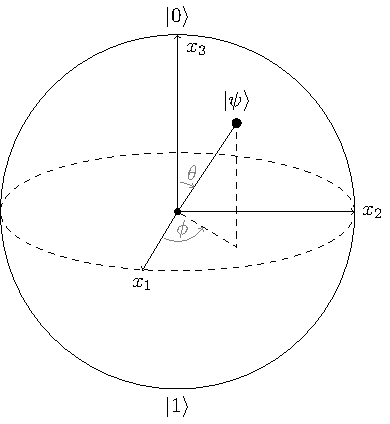
\includegraphics[width=0.7\textwidth]{images/quantum-information/bloch.pdf}
  \caption{Bloch-Kugel eines Qubits}\label{fig:bloch-sphere}
\end{figure}

Der Zustand des Qubits kann folgendermaßen berechnet werden:

\begin{equation}
  \ket{\psi} = \cos\frac{\theta}{2} \ket{0} + e^{i\phi} \sin\frac{\theta}{2} \ket{1}
\end{equation}

Ein Qubit kann also eine unendliche Anzahl an Zuständen annehmen.\footnote{Genaugenommen ist die Anzahl sogar \emph{überabzählbar}, also in einer höheren Unendlichkeisstufe als die natürlichen Zahlen.} Das ließe die die Vermutung zu, dass ein Qubit auch unendlich viele Informationen speichern kann. Dies ist jedoch nicht der Fall, weil beim Messen des Zustandes die Superposition zusammenfällt und das Qubit dann entweder den Wert $\ket{0}$ oder $\ket{1}$ hat.


\subsection{Codierung von Informationen}
\subsubsection{Verschränkung von Qubits}

Die eigentliche Stärke von Quantencomputern zeigt sich erst bei der Kombination mehrerer Qubits. Während ein einzelnes Qubit sich in einer Überlagerung der Zustände \(0\) und \(1\) befinden kann, erweitert sich der gesamte Zustandsraum beim Hinzufügen weiterer Qubits nicht nur additiv, sondern \emph{exponentiell}.

In klassischen Computern führen \(n\) Bits zu \(2^n\) möglichen Kombinationen von festen Zuständen, wobei sich zu jedem Zeitpunkt aber immer nur \emph{eine} dieser Kombinationen im Arbeitsspeicher befindet. Ein klassisches 3-Bit-System kann zum Beispiel genau einen dieser Zustände darstellen: \(000\), \(001\), ..., \(111\).

Ein Quantensystem aus \(n\) Qubits hingegen befindet sich in einer Superposition all dieser Zustände gleichzeitig. Es existieren also \(2^n\) sogenannte \emph{Basiszustände}, die gleichzeitig in der Beschreibung des Gesamtzustands mit bestimmten Gewichtungen (Wahrscheinlichkeitsamplituden) vorkommen. Der Gesamtzustand eines Qubit-Systems mit \(n\) Qubits kann somit als Superposition aller \(2^n\) möglichen klassischen Kombinationen dargestellt werden.

\[
\text{Zustandsraumdimension} = 2^n
\]

Zur Veranschaulichung:

\begin{itemize}
  \item Ein einzelnes Qubit: 2 Basiszustände (\(0\), \(1\))
  \item Zwei Qubits: 4 Basiszustände (\(00\), \(01\), \(10\), \(11\))
  \item Drei Qubits: 8 Basiszustände (\(000\), \(001\), ..., \(111\))
\end{itemize}

Jeder dieser Zustände kann gleichzeitig im Gesamtzustand des Systems enthalten sein – mit je einer komplexen Amplitude. Dies bedeutet nicht, dass der Quantencomputer alle Lösungen gleichzeitig kennt, aber dass er während der Berechnung in gewisser Weise mit vielen Möglichkeiten \emph{parallel} arbeiten kann. Dies ist ein wesentlicher Grund, warum manche Algorithmen auf Quantencomputern eine exponentielle Beschleunigung ermöglichen.

Je mehr Qubits man miteinander verschaltet, desto größer wird also der Zustandsraum. Schon mit wenigen Qubits lassen sich gewaltige Mengen an Zuständen darstellen:

\begin{table}[h]
\centering
\begin{tabular}{|c|c|}
\hline
\textbf{Anzahl Qubits} & \textbf{Mögliche Basiszustände} \\
\hline
1 & 2 \\
2 & 4 \\
3 & 8 \\
5 & 32 \\
10 & 1\,024 \\
20 & 1\,048\,576 \\
50 & \(\approx 1{,}13 \times 10^{15}\) \\
\hline
\end{tabular}
\caption{Exponentielles Wachstum der Zustandsanzahl mit zunehmender Qubit-Zahl}
\end{table}

Diese enorme Zustandsvielfalt ist nicht einfach direkt auslesbar – bei einer Messung kollabiert das Qubit-System zu genau einem dieser \(2^n\) Basiszustände. Dennoch erlaubt die gleichzeitige Verarbeitung dieser vielen Möglichkeiten innerhalb eines Algorithmus ein grundsätzlich neues Rechenparadigma.

\label{subsec:verschraenkungQubits}

\subsubsection{Fehlerkorrektur}
\subsubsection{Dense Coding}




\section{Quanten-Gatter}\label{sec:quanten_gatter}


\subsection{Ein-Qubit-Gatter}
Ein klassisches \emph{Ein-Bit-Gatter} nimmt einen einzelnen Bitwert als Eingabe und liefert einen Bitwert als Ausgabe. Sein Verhalten lässt sich durch eine Wahrheitstabelle angeben – etwa flippt das NOT-Gatter Eingaben $0 \rightarrow 1$ und $1 \rightarrow 0$. Abgesehen von der Identität ist NOT das einzige nicht-triviale Ein-Bit-Logikgatter der klassischen Welt. (Vgl. \cite[S.17f.]{nielsen_quantum_2010}) Ein \emph{Ein-Qubit-Gatter} transformiert dagegen den Zustand eines einzelnen Qubits. Strukturell handelt es sich um eine lineare, unitäre Abbildung im zweidimensionalen Zustandsraum. Konkret wird ein Ein-Qubit-Gatter durch eine $2\times 2$-Unitärmatrix $U$ beschrieben, die den Zustandsvektor des Qubits auf einen neuen Zustand abbildet. (Vgl. ebd., S. 174)

\begin{equation}
U = \begin{pmatrix}
a & b \\
c & d
\end{pmatrix}
\end{equation}
\\
Die Unitarität ($U^{\dagger}U = I$) stellt sicher, dass die Transformation physikalisch zulässig ist und rückgängig gemacht werden kann. Im Gegensatz zum klassischen Fall – mit nur einer nicht-trivialen Ein-Bit-Operation – existiert eine unendliche Vielfalt möglicher Ein-Qubit-Gatter, da jede $2\times 2$-unitäre Matrix ein gültiges Quantengatter repräsentiert. (Vgl. ebd.)\\
\\
In den folgenden Unterkapiteln \ref{subsec:pauli_gatter}, \ref{subsubsec:hadamard_gatter}, \ref{subsubsec:phase_shift_gatter} werden die in der folgenden Abbildung dargestellten Ein-Qubit-Gatter näher erläutert:


%https://www.tfp.kit.edu/downloads/lehre_2013_ss/aaa_HSS13_Grundlagen.pdf, Folie 13 --> Nur inspiriert, denke, dass kein Zitat notwendig ist

\newcommand{\gatterbox}[1]{%
  \tikz[baseline=-0.5ex]{
    \draw[-] (-1,0) -- (-0.3,0);
    \draw[thick] (-0.3,-0.4) rectangle (0.3,0.4);
    \node at (0,0) {\( #1 \)};
    \draw[-] (0.3,0) -- (1,0);
  }%
}
\[
\begin{array}{c@{\hspace{1cm}}c@{\hspace{1cm}}c}
\textbf{Pauli-X/Y/Z-Gatter} & \textbf{Hadamard-Gatter} & \textbf{Phase-Shift-Gatter} \\
\gatterbox{X} & \gatterbox{H} & \gatterbox{R_\Theta}
\end{array}
\]


\subsection{Pauli-Gatter $X$, $Y$, $Z$}\label{subsec:pauli_gatter}

Die Pauli-Matrizen wurden erstmals 1927 von dem Physiker Wolfgang Pauli eingeführt, um den neu entdeckten Elektronenspin im Rahmen der Quantenmechanik zu beschreiben. Elektronen besitzen einen intrinsischen Drehimpuls (Spin ½), der keine klassische Entsprechung hat. (Vgl. \cite[S.312]{wekesa_sirengo_mathematical_2024}) Pauli entwickelte drei $2\times 2$-Matrizen (oft $\sigma_x, \sigma_y, \sigma_z$ bezeichnet), um die Spin-$x$-, Spin-$y$- und Spin-$z$-Operatoren des Elektrons darzustellen. Dies geschah im Kontext der Erklärung des anomalous Zeeman-Effekts, bei dem Spektrallinien in Magnetfeldern aufgespalten werden – ein Phänomen, das mit dem zusätzlichen Freiheitsgrad des Elektronenspins erklärt werden konnte. (Vgl. ebd.)\\
\\
Die Pauli-Gatter $X$, $Y$, $Z$ sind die meistverwendeten Ein-Qubit-Gatter. In der üblichen Darstellungsform (der sogenannten $Z$-Basis ${|0\rangle,|1\rangle}$) lauten sie:
\\


\begin{equation}
  X=\begin{pmatrix}0&1\\ 1&0\end{pmatrix},\qquad
  Y=\begin{pmatrix}0&-i\\ i&0\end{pmatrix},\qquad
  Z=\begin{pmatrix}1&0\\ 0&-1\end{pmatrix}.
\end{equation}
Jede Matrix ist dabei \emph{unitär}: Multipliziert man sie mit ihrer konjugiert-transponierten Version, erhält man wieder die Einheitsmatrix. (Vgl. \cite[S.71]{nielsen_quantum_2010}) Außerdem ist sie \emph{hermitesch}: Die Matrix ist ihr eigenes „Spiegelbild“. (Vgl. ebd., S.78) Beides zusammen heißt, wenn man ein Pauli-Gatter zweimal anwendet, steht das Qubit wieder da, wo es zuvor war ($U^2=I$). Es ergeben sich dabei ausschließlich die Eigenwerte $+1$ oder $-1$. Damit besitzt jeder Pauli-Operator genau zwei orthogonale Eigenzustände, was ihn zum einfachsten nicht-trivialen Messoperator macht. Weiterhin sind die Pauli-Matrizen spurlos, d.h. ihre Spur (die Summe der Diagonalelemente) ist Null. (Vgl. ebd., S.76)\\
\\
Jeder Qubit-Zustand lässt sich wie in Unterkapitel \ref{subsec:blockkugel} als Punkt auf einer Einheitskugel darstellen. In diesem Bild wirken die Pauli-Gatter wie Halbumdrehungen um die drei Raumachsen: $X$ rotiert den Bloch-Vektor um $180^{\circ}$ um die $x$-Achse, $Y$ um die $y$-Achse und $Z$ um die $z$-Achse. (Vgl. \cite[S.215ff.]{rieffel_quantum_2011}) Die Eigenzustände von $Z$ liegen daher an Nord- und Südpol, während die Eigenzustände von $X$ und $Y$ entlang des Äquators auf den $x$- bzw.\ $y$-Achsen sitzen.\\
\\
Die Wirkung der Ein-Quibit-Gatter Pauli-$X$-, $Y$-, $Z$-Gatter wird folgendermaßen beschrieben:



\begin{itemize}
\item Pauli-$X$ (Bit-Flip-Gatter): Vertauscht die Basiszustände $|0\rangle$ und $|1\rangle$. Formal gilt $X|0\rangle = |1\rangle$ und $X|1\rangle = |0\rangle$. (Vgl. ebd., S.81-82) Dieses Gatter entspricht somit einem quantenmechanischen NOT-Operator – analog zum klassischen Inverter (NOT-Gatter) flipping eines Bits. Aufgrund dieser Wirkung wird $X$ auch als Bitflip-Operator bezeichnet. 

\item Pauli-$Y$ (kombiniertes Gatter): $Y$ lässt sich als $Y = iZ \cdot X$ auffassen. Entsprechend kombiniert es eine Bit-Flip- und eine Phasenflip-Operation. Konkret gilt $Y|0\rangle = \mathrm{i},|1\rangle$ und $Y|1\rangle = -,\mathrm{i},|0\rangle$ (mit $\mathrm{i}=\sqrt{-1}$). Man sieht, dass $Y$ – ähnlich wie $X$ – $|0\rangle$ und $|1\rangle$ vertauscht, jedoch zusätzlich einen komplexen Phasenfaktor ($\pm,\mathrm{i}$) hinzufügt. (Vgl. ebd.) Im Ergebnis ist $Y$ somit ein Bit-Flip mit Phasendrehung und wird manchmal auch als kombiniertes Bit- und Phasenflip-Gatter bezeichnet.

\item Pauli-$Z$ (Phase-Flip-Gatter): Lässt $|0\rangle$ invariant und kehrt die Phase von $|1\rangle$ um. Das heißt, $Z|0\rangle = |0\rangle$, aber $Z|1\rangle = -,|1\rangle$. In einem Superpositionszustand $a|0\rangle + b|1\rangle$ bewirkt $Z$ also einen Phasenfaktor $-1$ für den $|1\rangle$-Anteil. (Vgl. ebd.) Dieses Verhalten – ein Vorzeichenwechsel für einen der Basiszustände – erklärt die Bezeichnung Phasenflip-Gatter.
\end{itemize}\\
\\
Die Pauli-Gatter sind in Quantenlogik-Schaltkreisen äußerst wichtig. (Vgl. ebd., S. 81) Sie gehören meist zur Grundmenge der verfügbaren elementaren Quantenoperationen auf einem Qubit. Zusammen mit dem Einheitsoperator $I$ bilden sie die sogenannte Pauli-Gruppe auf einem Qubit, welche eine Rolle in vielen Quantum-Circuit-Konstruktionen spielt. Komplexere Ein-Qubit-Gatter lassen sich oft durch Kombinationen der Pauli-Gatter darstellen. So ist etwa das weit verbreitete und im folgenden Unterkapitel \ref{subsubsec:hadamard_gatter} beschriebenen Hadamard-Gatter eine von den Pauli-Matrizen abgeleitete Transformation (z.B. als $H = \frac{X+Z}{\sqrt{2}}$). Auch Kontrollgatter wie CNOT können unter Nutzung von Pauli-Operatoren konstruiert werden. (Vgl. \cite[S.312]{wekesa_sirengo_mathematical_2024})\\
\\

\subsection{Hadamard-Gatter}\label{subsubsec:hadamard_gatter}

Das Hadamard-Gatter $H$ ist das wohl einfachste Mittel, um aus einem klassischen Qubit-Zustand eine echte Überlagerung (Superposition) zu erzeugen.  Während ein Bit nur entweder 0 oder 1 sein kann, vermischt $H$ die beiden Basiszustände so, dass das Qubit  „halb 0, halb 1“ wird. (Vgl. \cite[S.19f.]{nielsen_quantum_2010})\\
\\
Formal schreibt man (Vgl. \cite[S.76]{rieffel_quantum_2011}).
\\
\begin{equation}
  H = \frac1{\sqrt2}\!
  \begin{pmatrix} 1 & 1 \\ 1 & -1 \end{pmatrix},
  \qquad
  H|0\rangle=\frac{|0\rangle+|1\rangle}{\sqrt2},
  \quad
  H|1\rangle=\frac{|0\rangle-|1\rangle}{\sqrt2}.
\end{equation}
\\
Die beiden resultierenden Zustände $|+\rangle$ und $|-\rangle$ liegen genau auf der Äquatorebene der Bloch-Kugel; $H$ entspricht dort einer $\pi$-Drehung um die Achse $\tfrac{x+z}{\sqrt2}$ (Vgl. ebd., S.22).\\
\\
Da $H$ involutorisch ist ($H^2=I$), kehrt eine zweite Hadamard-Operation den Prozess exakt um.  Dies erklärt die populäre Kurzformel „$H$ ist die \emph{square-root of NOT}“ (Vgl. \cite[S.19f.]{nielsen_quantum_2010}): einmal angewendet bewirkt es einen halben Bit-Flip (Superposition), zweimal angewendet ergibt sich der volle Flip zurück zum Ausgangszustand.\\
\\
Die Fähigkeit, Superpositionen mit nur einem Gate herzustellen, macht $H$ unverzichtbar für viele Quantenalgorithmen.  Im Deutsch-Jozsa-Algorithmus oder in Grovers Suche präpariert $H^{\otimes n}$ aus $|00\ldots0\rangle$ eine gleichgewichtige Überlagerung aller $2^{n}$ Eingabewerte und ermöglicht so Quantenparallelismus (Vgl. ebd., S. 250ff.).  Ohne ein solches Gate gäbe es keine Interferenzeffekte und folglich keinen Geschwindigkeitsvorteil gegenüber klassischer Berechnung.

%\subsection{Phase-Shift-Gatter}\label{subsubsec:phase_shift_gatter}


\subsection{Mehr-Qubit-Gatter}


\subsection{SWAP}



\subsection{CNOT}


%\subsection{CU-Gatter}


%\subsection{Quantenschaltungen}


\section{TBD: Erste Algorithmen}
Algorithmen in der klassischen Informatik basieren alle auf einer linearen, schrittweisen Verarbeitung von Daten. So kann ein Bit, mit dem Wert 1 in einem folgenden Rechenschritt entweder den Wert 0 annehmen oder seinen aktuellen Wert 1 behalten. In einem Quantencomputer hingegen, kann das QBit nach einer Transformation unendlich viele verschiedene Werte annehmen.\\
\\
Mit dem Wissen aus vorherigen Kapitel lassen sich bereits die ersten, einfachen Quantenalgorithmen entwerfen, welche theoretisch schneller auf Quantencomputer ausgeführt werden können oder sogar für klassische Computer unmöglich sind zu lösen. \\
\\
Dazu beleuchten wir die Herkunft moderner Quantencomputer und die ersten Quantenalgorithmen.

\subsection{TBD: Touring Complete} 
In einem Paper von 1985 stellt der Physiker David Deutsch die Idee eines universellen Quantencomputers vor. Dabei verbindet er Quantenmechanik mit der theoretischen Informatik und kritisiert die klassische Church-Turing-These, da sie physikalisch nicht vollständig sei. Er schlägt stattdessen die Church–Turing–Deutsch-These vor: Alles, was physikalisch berechenbar ist, kann von einem Quantencomputer simuliert werden.\\
\\
Zentral im Paper ist der Vorschlag eines konkreten Quantenalgorithmus, welcher heute als der Deutsch-Algorithmus bekannt ist. Dieser zeigt, dass Quantencomputer Probleme effizienter lösen können als klassische Rechner.  (Vgl. \cite{deutsch_quantum_1985})\\

\subsection{Algorithmus von Deutsch} 
Gegeben ist eine binäre Funktion $f:\{0,1\} \rightarrow \{0,1\}$. Man möchte herausfinden, ob $f$ konstant (d.h. $f(0)=f(0)$) oder balanciert (d.h. $f(0)\neq f(0)$) ist.\\
\\
Klassisch muss man beide Werte $f(0)$ und $f(1)$ abfragen. Deutsch zeigt, dass ein Quantencomputer mit nur einer Abfrage an ein Quanten-Orakel die Antwort liefern kann. Ein Quantenorakel ist dabei eine unbelichtete Funktion, welche $n$-Bits als Eingabe und $m$-Bits als Ausgabe liefert. Man könnte das Orakel auch als "Black Box" bezeichnen, deren Funktionsweise nicht nachvollziehbar ist. \\
\\
Um das Problem von Deutsch zu lösen, müssen wir eines der Quantenbits in eine Superposition über beide möglichen Eingaben von $f$ versetzten.\\
\\
Alle Rechenschritte müssen umkehrbar sein. Da $f$ in dem konstanten Fall nicht reversible ist muss ein zweites Quantenbit für den Algorithmus verwenden. Daraus ergibt sich folgender Funktionsaufruf. 

$$
U_f: \left|x\right\rangle\left|, y\right\rangle \rightarrow  \left|x, y \oplus f(x)\right\rangle
$$\\
\\
Jetzt kann auf das Problem der Algorithmus von Deutsch angewendet werden. Dieser löst das Problem in folgenden 4 Schritten:

\begin{enumerate}
    \item Initialzustand: Zwei QBits im Zustand
$$\left|x\right\rangle\left|y\right\rangle \leftarrow  \left|0\right\rangle \left|1\right\rangle$$
\item Anwenden des Hadamard-Gatters auf beide QBits erzeugt Superposition:
$$
\left|x\right\rangle\left|y\right\rangle \leftarrow  H\left|x\right\rangle H\left|y\right\rangle
$$
\item Anwendung des Orakels $U_f$:
 $$
\left|x\right\rangle\left|y\right\rangle \leftarrow  U_f\left|x\right\rangle\left|y\right\rangle
$$
	Durch die vorbereitete Superposition des Zielregisters wird die Funktion $f(x)$ in die Phase codiert.
\item Nach erneuter Hadamard-Transformation misst man:
	- Hat $\left|x\right\rangle\left|y\right\rangle$ den Wert $\left|0\right\rangle\left|1\right\rangle$: Funktion ist konstant
	- Hat $\left|x\right\rangle\left|y\right\rangle$ den Wert $\left|1\right\rangle\left|1\right\rangle$: Funktion ist balanciert

\end{enumerate}

Daraus folgt der Schaltkreis in Abbildung \ref{fig:deutsch-schaltkreis}.
\begin{figure}
    \centering
    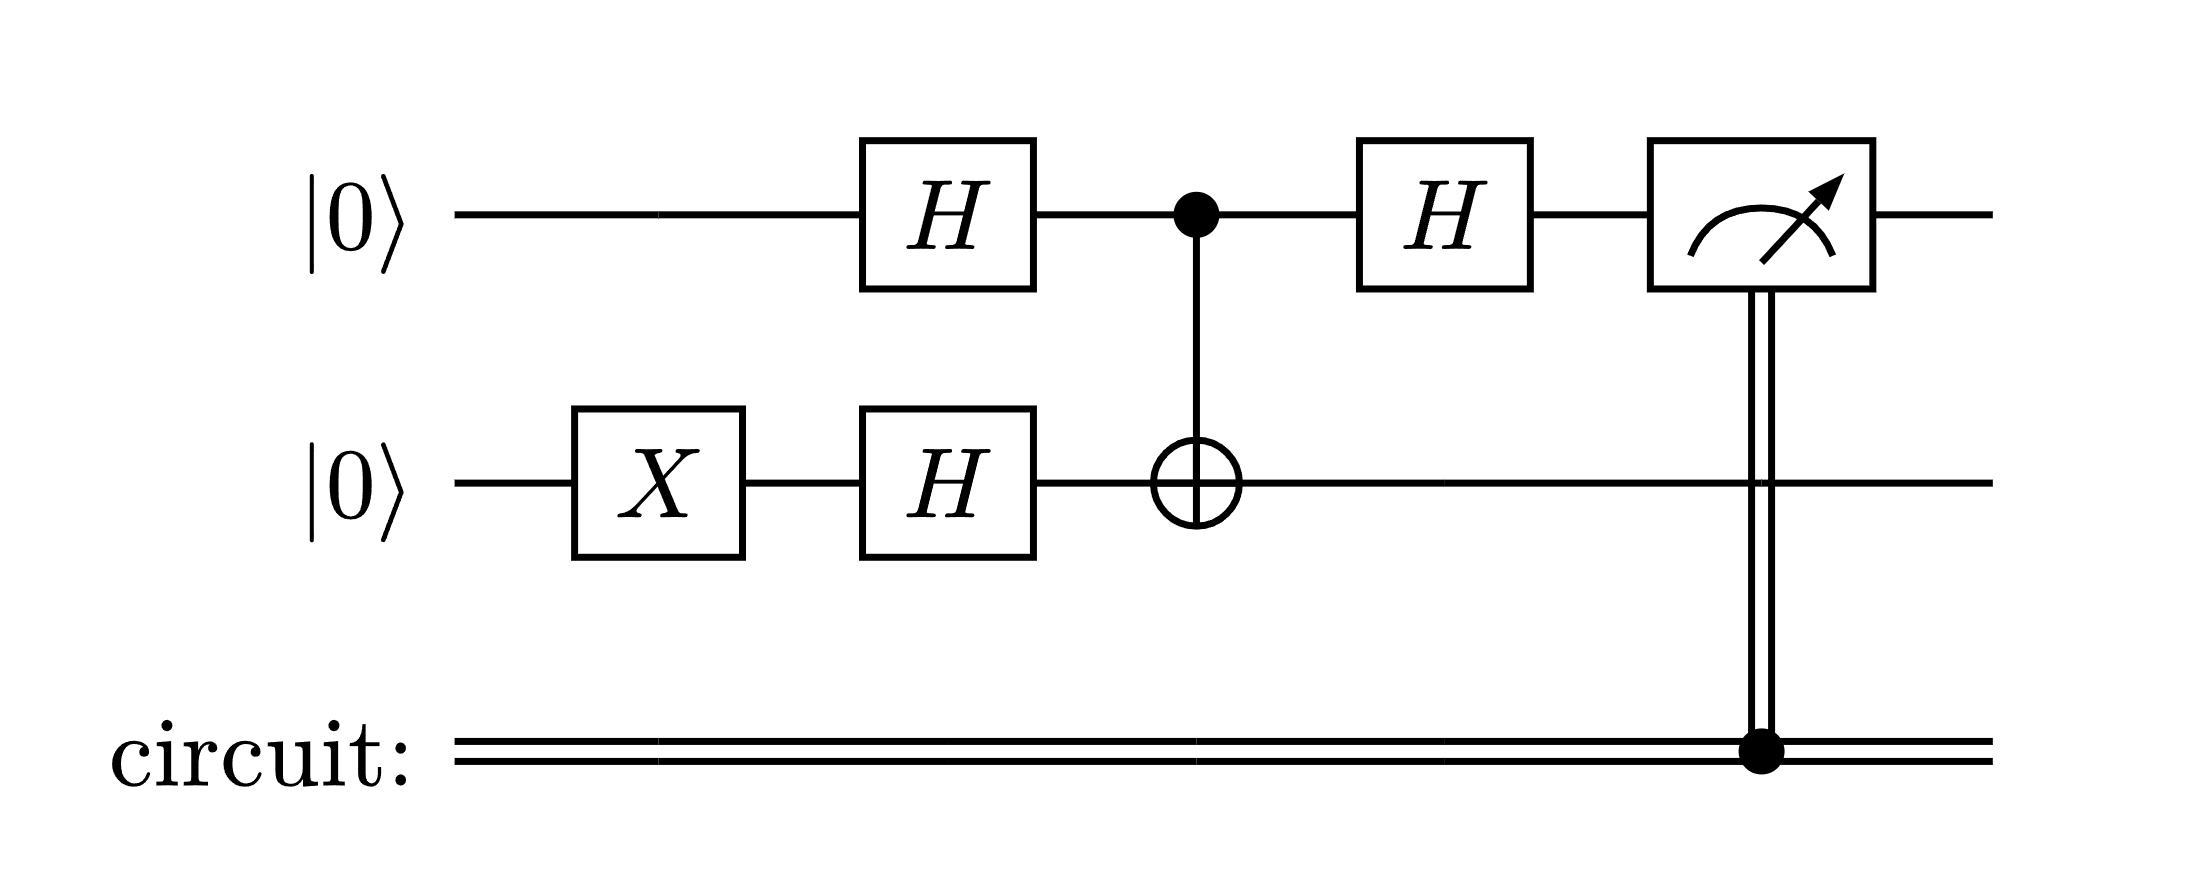
\includegraphics[width=1\linewidth]{images//quantum-information/deutsch schaltkreis.png}
    \caption{Schaltkreis: Deutsch-Algorithmus}
    \label{fig:deutsch-schaltkreis}
\end{figure}

Somit liefert Deutsch den ersten Beweis für Quantenparallelität durch Superpositionen in einem konkreten Algorithmus. Der von Deutsch vorgeschlagene Algorithmus ermöglicht es jedoch nur Probleme mit einem einzigen Eingabe Bit zu verarbeiten. Eine verallgemeinerte Version des Deutsch-Algorithmus lieferte David Deutsch zusammen mit Richard Jozsa ein paar Jahre später in dem Paper "Rapid solution of problems by quantum computation". (Vgl. \cite[S.33-37]{homeister_quantum_2022})

\subsection{Deutsch-Josza Algorithmus}
Reale Probleme haben meist deutlich komplexere Strukturen und benötigen mehr Eingabebits als eines. Um diesem Umstand gerecht zu werden, entwickelten David Deutsch und Richard Jozsa eine Verallgemeinerung, welche als Deutsch-Jozsa-Algorithmus bekannt ist. Dieser erlaubt es, Funktionen mit beliebig vielen Eingabebits zu untersuchen und demonstriert erstmals einen exponentiellen Vorteil gegenüber klassischen Computern.\\
\\
Genau wie bei dem Deutsch-Algorihmus ist eine Funktion $f:\{0,1\}^n \rightarrow \{0,1\}$ gegeben. Dieses mal aber mit $n$-Bits als Eingabe. $f$ ist entweder konstant oder balancier. Da es nun jedoch mehrere Eingabebits gibt, bedeutet Balanciert, dass genau die Hälfte aller möglichen Ausgaben $0$ und die andere Hälfte $1$ als Ergebnis liefert. (Vgl. \cite{deutsch_rapid_1992})\\
\\
Das Ziel bleibt unverändert. Es soll mit möglichst wenig Abfragen bestimmt werden, welcher der beiden Fälle vorliegt. Klassische Algorithmen benötigen für das Problem im schlimmsten Fall $2^{n-1}+1$ Abfragen, um Gewissheit zu erlangen. \\

Der Algorithmus läuft in folgenden Schritten ab:

\begin{enumerate}
\item Initialzustand:  Ein Register mit $n$ QBits im Zustand $\left|0\right\rangle^{\otimes n}$ und ein Hilfs-QBit im Zustand $\left|1\right\rangle$
\item Hadamard-Transformation auf alle QBits erzeugt eine Superposition:
$$
\left|x\right\rangle\left|y\right\rangle \leftarrow  H^{\otimes n}\left|0\right\rangle^{\otimes n} \otimes H\left|1\right\rangle
$$
\item Anwendung des Orakels $U_f$, das kohärent alle $2^n$ Eingaben verarbeitet:
$$
U_f \left|x\right\rangle\left|y\right\rangle = \left|x\right\rangle\left|y \oplus f(x)\right\rangle
$$
    Wie beim Deutsch-Algorithmus wird $f(x)$ in die Phase des Zustands eingeschrieben.
\item Erneute Hadamard-Transformation auf die ersten $n$ QBits.
\item Messung:
    \begin{itemize}
      \item Ergebnis $\left|0\right\rangle^{\oplus n}$ bedeutet die Funktion ist konstant
      \item Jedes andere Ergebnis bedeutet Funktion ist balanciert
    \end{itemize}
\end{enumerate}

Abbildung \ref{fig:deutsch-jozsa-schaltung} zeigt einen entsprechenden Quantenschaltkreis mit 4 QBits. 
\begin{figure}
    \centering
    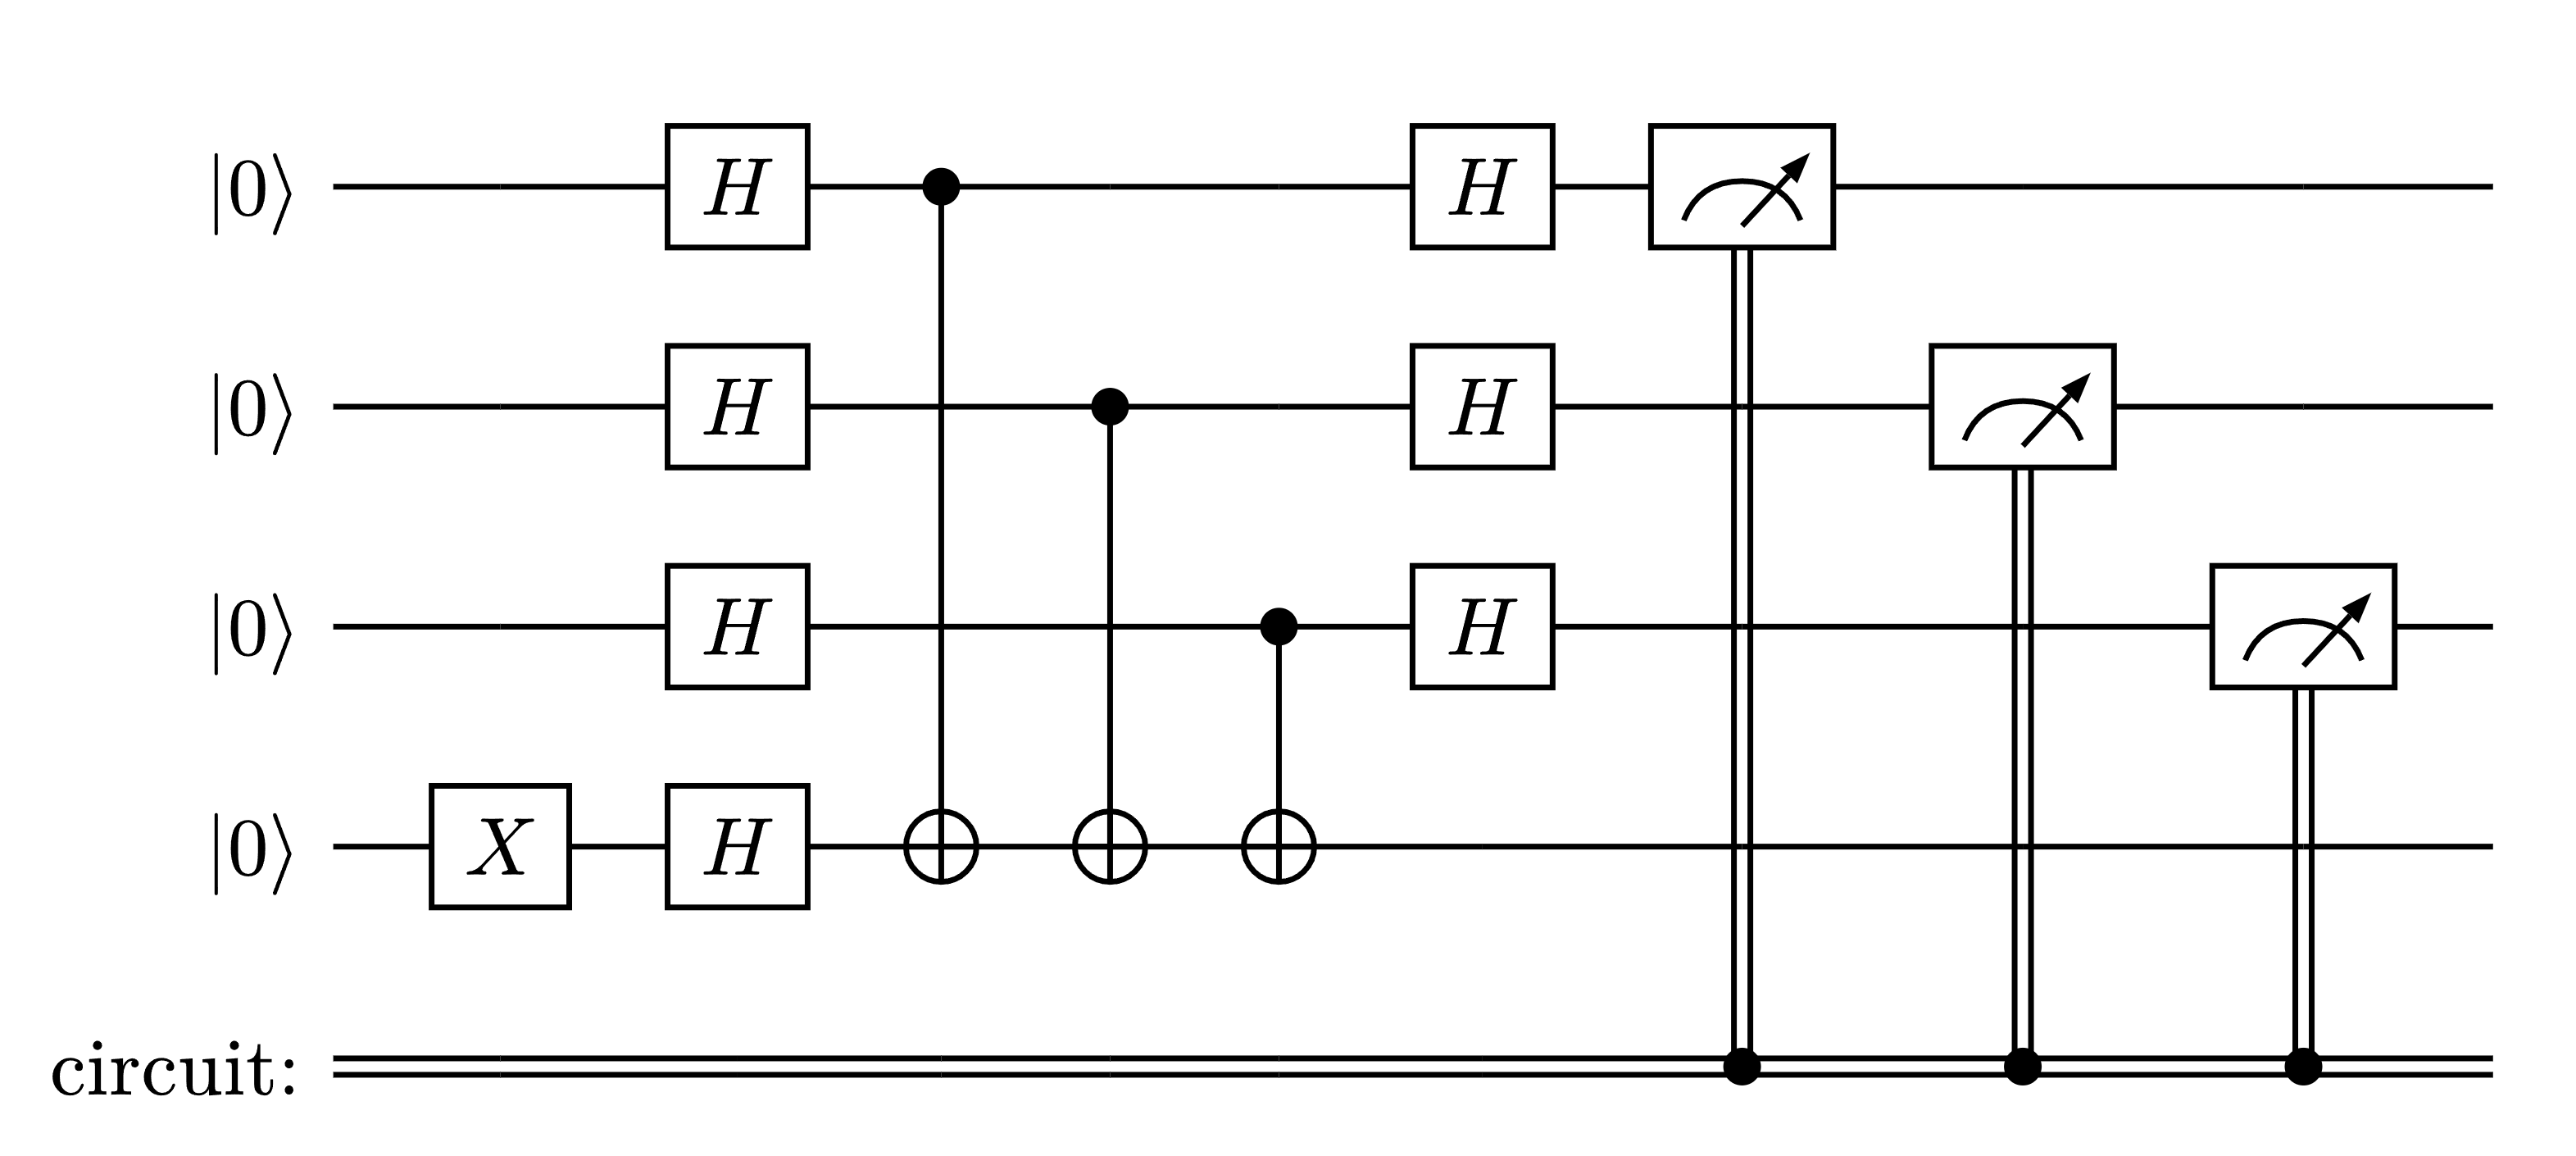
\includegraphics[width=1\linewidth]{images//quantum-information/deutsch-jozsa schaltkreis.png}
    \caption{Schaltkreis: Deutsch-Jozsa Algorithmus}
    \label{fig:deutsch-jozsa-schaltung}
\end{figure}

Das Besondere an dem Algorithmus ist, dass er das Ergebnis deterministisch und ohne Wahrscheinlichkeiten nach nur einer einzigen Orakelabfrage liefert. Durch Interferenz löschen sich bei balancierter Funktion die Amplituden für $\left|0\right\rangle^{\oplus n}$ vollständig aus. Nur im konstanten Fall bleibt sie erhalten. Somit liefert Deutsch und Jozsa den ersten theoretischen Beweis, dass Quantencomputer bei bestimmten Problemen klassischen Computern exponentiell überlegen sein können. (Vgl. \cite[S.62-66]{homeister_quantum_2022})





\section{Quantenverschränkung und Teleportation}

\subsection{Quantenverschränkung}
Die Quantenverschränkung ist ein Phänomen, bei dem zwei oder mehr Quantenobjekte sich in einem Zustand befinden, in dem sie, egal wie weit voneinander entfernt sie sind, gleich auf externe Reize reagieren. Solche Objekte, bei denen die Quantenverschränkung nachgewiesen werden konnte, sind Atome, Elementarteilchen wie Elektronen und Photonen, bis hin zu Kristallen.\\
\\
An einem Beispiel mit Elektronen lässt sich die Quantenverschränkung wie folgt erklären. Elektronen können sich in einem Zustand befinden, in dem sie keine eindeutige, exakte Position haben, sondern eine Menge an potentiellen Positionen. Diese potentiellen Positionen befinden sich alle im Umfeld der durchschnittlichen Position, dem Massenmittelpunkt des Elektrons, wie eine Wolke. Wenn von diesem Elektron seine Position gemessen wird, antwortet dieses Elektron auf die Messung mit einem zufälligen Wert. Bei den nächsten Messungen wird wiederum mit einem anderen zufälligen Wert geantwortet. Es besteht ein Indeterminismus. In diesem Zustand ist es sogar möglich, dass sich das Elektron, wegen dem Indeterminismus auch an zwei oder mehr Positionen gleichzeitig befindet. Und dieses Elektron, an zwei oder mehr Positionen gleichzeitig, reagiert auf Reize auf die gleiche Weise. Dies wurde im Doppelspaltexperiment von Thomas Young nachgewiesen, bei dem ein Elektron auf einen Reiz an der ersten Position an einem Young‘schen Spalt reagiert, und auf einen Reiz an der zweiten Position an einem anderen Young’schen Spalt reagiert.\\
\\
Obwohl es möglich ist, dass ein Quantenobjekt keine exakte Position hat, und ein weiteres mit dem ersten Quantenobjekt verbundenes, „verschränktes“ Quantenobjekt ebenfalls keine eindeutige Position hat, ist die Distanz zwischen den beiden Quantenobjekten klar bestimmt. Wenn man also die Position der beiden Quantenobjekte misst, erhält man für beide immer einen zufälligen Wert. Aber die Differenz der zufälligen Werte voneinander ist immer genau gleich. Das gilt immer, auch wenn die beiden Quantenobjekte sehr weit voneinander entfernt sind. Die Position eines Quantenobjekts selbst ist nicht wohlbestimmt, die Position im Bezug auf ein verbundenes, verschränktes Quantenobjekt hingegen schon. Dass sich ein Quantenobjekt „hier“ und „einer festen Distanz von hier“ gleichzeitig befindet, wird „Superposition“ genannt. Und dieser superpositionierte Zustand ist ein verschränkter Zustand.\\
\\
Die Verschränkung fixiert nicht nur die Distanz von zwei oder mehr Quantenobjekten voneinander, sondern auch weitere Variablen, z.B. die Geschwindigkeit. Sie haben die gleiche Geschwindigkeit, welche aber selbst nicht fest ist, sondern eine von einer Menge potentieller Geschwindigkeiten.\\
\\
(Vgl. \cite[S.83-88]{gisin_unbegreifliche_2014}) 

\subsection{Quantenteleportation: Protokoll, um einen unbekannten Quantenzustand mithilfe eines verschränkten Paares und klassischer Kommunikation zu übertragen}
Ein Objekt besteht aus Materie und physikalischem Zustand. Bei Quantenobjekten ist die Materie die Masse und permanente Attribute wie z.B. die elektrische Ladung bei Elektronen, bzw. die Energie bei massenlosen Quantenobjekten wie z.B. Photonen. Der physikalische Zustand ist gebildet aus potentiellen Attributen, wie z.B. die potentiellen Positionen (denke Wolke um Massen-/ Energiemittelpunkt), die potentiellen Geschwindigkeiten bei Elektronen bzw. die potentiellen Schwingungsfrequenzen bei Photonen.\\
\\
In der Quantenteleportation wird der Zustand eines Quantenobjekts, der sog. Quantenzustand, ohne das Durchlaufen einer Zwischenstrecke, von einer Position auf eine andere Position, vorausgesetzt, dass sich in dieser anderen Position ein Quantenobjekt derselben Art befindet, direkt versetzt. Die Masse bzw. Energie kann nicht teleportiert werden, weil dies das Prinzip der Unmöglichkeit von Kommunikation ohne Signalübertragung verletzen würde. Dahingegen hat der Zustand weder eine Masse, noch eine Energie, denn sie ist potentiell – eine Wahrscheinlichkeit.\\
\\
Nach einer solchen Quantenteleportation verliert das Quantenobjekt seinen Zustand. Am Beispiel eines Photons kann man dies wie folgt erklären. Es gebe ein Photon mit gut strukturierter Polarisation. Bei solch einem Photon schwingt das elektrische Feld regelmäßig in eine bestimmte Richtung. Nach der Quantenteleportation verliert dieses Photon seine Struktur. Übrig bleibt ein depolarisiertes Photon, ein Photon mit strukturloser Polarisation, dessen elektrisches Feld unregelmäßig in alle Richtungen schwingt. Der Quantenzustand des ersten Quantenobjekts nach der Quantenteleportation entspricht dem Quantenzustand des zweiten Quantenobjekts vor der Quantenteleportation.\\
\\
Der Quantenzustand, der teleportiert wird, ist ein Qubit. Voraussetzung einer Quantenteleportation ist das Dasein einer Menge verschränkter Quantenobjekte. In der nächsten Subsektion wird hierüber genauer erläutert.\\
\\
(Vgl. \cite[S.124-128]{gisin_unbegreifliche_2014}) 


\subsection{Bennett und Brassard (1993): wie drei Qubits (Senderzustand + 2 verschränkte) genutzt werden, um den Zustand über Distanz zu „teleportieren“}
Es gebe ein Quantenobjekt eines Senders mit unbekanntem Quantenzustand bzw. Qubit \(\ket{\Phi}\). Dieser Qubit soll zu einem dritten Quantenobjekt eines Empfängers teleportiert werden. Der Sender ist im Besitz eines zweiten Quantenobjekts mit dem ursprünglichen Zustand \(\ket{\alpha_0}\), „Ancilla“ bzw. „Ancilla-Qubit“ genannt. Im ersten Schritt der Quantenteleportation bringt der Sender das Quantenobjekt mit dem Qubit \(\ket{\Phi}\) und das Quantenobjekt mit dem Ancilla-Qubit dazu, so miteinander zu interagieren, dass das erste Quantenobjekt in einen Standard Zustand \(\ket{\Phi_0}\), und das zweite Quantenobjekt in einen unbekannten Quantenzustand \(\ket{\alpha}\), welches die vollständige Information über \(\ket{\Phi}\) enthält, versetzt wird. Diese Interaktion ist eine gemeinsame Messung der Quantenzustände beider Quantenobjekte des Senders. Allerdings muss erwähnt werden, dass eine solche Messung nur ein positives Ergebnis liefert, wenn der Qubit \(\ket{\Phi}\) einem orthonormalen Set angehört. Im zweiten Schritt der Quantenteleportation wird dann die neue Ancilla, bzw. in anderen Worten das (positive) Ergebnis der Messung im ersten Schritt, an das Quantenobjekt des Empfängers gesendet, wonach der Empfänger die Qubit-Veränderung auslösende Interaktion vom Sender rückgängig machen kann, und somit eine Replikation des originalen Quantenobjekts mit dem Qubit \(\ket{\Phi}\) herstellen kann. Auf dieser Weise können Informationen von Quantenobjekten, also Quanteninformationen, ausgetauscht werden, ohne dass ein Quantenobjekt geklont wird. Diese Methode der Quantenteleportation wird „spin-exchange“ genannt.\\
\\
(Vgl. \cite[S.1-2]{bennett_teleporting_1993})\\
\\
Am anfänglichen Zustand der „spin-exchange“ Methode sind das Quantenobjekt 2 auf der Senderseite und das Quantenobjekt 3 auf der Empfängerseite miteinander verschränkt. Durch die Interaktion auf Senderseite, wobei die Qubits der Quantenobjekte 1 und 2 verändert werden, wird die Verschränkung der Quantenobjekte 2 und 3 aufgehoben, und stattdessen die Quantenobjekte 1 und 2 verschränkt.\\
\\
(Vgl. \cite[S.2-3]{bennett_teleporting_1993})\\
\\
Mathematisch lässt sich der Prozess, wobei die Quantenobjekte in diesem Beispiel spin-\(\frac{1}{2}\) Partikel sind, mit folgenden Formeln darstellen:

\[ \ket{\Psi_{23}^{(-)}} = \sqrt{\frac{1}{2}} (\ket{\uparrow_2}\ket{\downarrow_3} + \ket{{\downarrow_2}\ket{\uparrow_3}}) \]
\\
Das zweite Quantenobjekt vom Sender (2) und das Quantenobjekt vom Empfänger (3) befinden sich in einem verschränkten Zustand. Dies ist die Ausgangssituation.

\[ \ket{\Psi_{12}^{(+)}} = \sqrt{\frac{1}{2}} (\ket{\uparrow_1}\ket{\downarrow_2} + \ket{{\downarrow_1}\ket{\uparrow_2}}) \]
\[ \ket{\Phi_{12}^{(\pm)}} = \sqrt{\frac{1}{2}} (\ket{\uparrow_1}\ket{\uparrow_2} \pm \ket{{\downarrow_1}\ket{\downarrow_2}}) \]
\\
Nun findet die gemeinsame Messung der beiden Quantenobjekte des Senders statt. Die vier sich in den Formeln befindenden Zustände bilden eine orthonormale Basis für die Quantenobjekte 1 und 2. Hiermit ist die Verschränkung der Quantenobjekte 2 und 3 aufgehoben, und stattdessen sind 1 und 2 verschränkt.

\[ \ket{\Phi} = \ket{\Phi_1} = a{\uparrow_1} + b{\downarrow_1} \]
\\
Für einfache Verständlichkeit wird der unbekannte Originalzustand von Quantenobjekt 1, \(\ket{\Phi}\), so geschrieben. Dabei ist \(|a|^2 + |b|^2 = 1\).\\
\\
(Vgl. \cite[S.2]{bennett_teleporting_1993})

\subsection{Quantenkommunikation per Quantenverschränkung in Quantennetzwerken}
In der Quantenkommunikation bzw. im Quanteninformationstransfer innerhalb eines Quantennetzwerks werden Qubits bzw. Quantenzustände über Quantenkanäle gesendet. Quantenkanäle verbinden entfernte Knoten in einem Quantennetzwerk. Diese Quantenkanäle haben eine sog. Absorptionslänge. Die Länge der Quantenkanäle, und damit die maximale Distanz zweier miteinander verbundenen Knoten in einem Quantennetzwerk, ist nur auf wenige Vielfache der Absorptionslänge begrenzt. Dies führt zum Problem, dass Quantenkanäle „eng“ und „laut“ (Originaltext „noisy“) sind, und die transportierten Qubits sich miteinander verschränken können, was zu einem Übertragungsfehler führen könnte.\\
\\
Eine Lösung, die Wahrscheinlichkeit solcher Übertrangungsfehler zu reduzieren, mit Hinnahme von einer größeren Menge an benötigten Ressourcen, ist es, einzelne Qubits in einen konkatenierten Quantencode (z.B. einen verschränkten Zustand einer Vielzahl von Qubits) zu kodieren, und Operationen an diesem Code durchzuführen, während es durch den Quantenkanal übertragen wird. Dies wird „Verschränkungsreinigung“ (vom Eng. „entanglement purification“) genannt und ermöglicht möglichst unverfälschten Quanteninformationstransfer und sichere Quantenkryptographie in „engen“ und „lauten“ Quantenkanälen.\\
\\
Und um unverfälschten Quanteninformationstransfer auch über längere Quantenkanäle sicherzustellen, kann ein Schema verwendet werden, wobei sog. „Quantenrepeater“ einen langen Quantenkanal in kürzere Segmente aufteilen, und die Verschränkungen separat bereinigen, bevor diese wieder aneinander gehängt werden. Im Übergang von einem Segment zum nächsten werden Quantenkorrelationen aufgebaut, basieren auf Korrelationen die innerhalb der einzelnen Segmente existieren.\\
\\
(Vgl. \cite[S.1-2]{dur_quantum_1999})

\subsection{Quantenteleportation in Quantencomputern}
Für folgende Abschnitte gilt die Quelle (Vgl. \cite[S.1-2]{gottesman_quantum_1999}).\\
\\
Die Wissenschaftler Daniel Gottesman und Isaac Chuang stellen eine Technik, eine Verallgemeinerung von Quantenteleportation vor, welche Quantenberechnung in Quantencomputern effizient und ressourcenarm zulässt, und dabei bekannte fehlertolerante Protokolle für Quantenberechnung vereinigt. Mit dieser Technik der Quantenteleportation sollen Quanteninformationen in einen neuen Zustand transformiert werden, was der Wirkung eines Quantengatters ähnelt.\\
\\
Zwei Qubits werden durch ein CNOT (controlled NOT) Gatter (gate) teleportiert. Ein CNOT gate ist eine Komponente, die zwei verschränkte Qubits in einem Bell-Zustand aufnimmt und den zweiten Qubit, den sog. „target“ Qubit dreht, wenn der erste Qubit, der sog. „control“ Qubit, einen Wert von \(\ket{1}\) hat. Beim Durchgang werden Pauli-Matrix Operationen durchgeführt, welche die Quanteninformationen, also den Quantenzustand, auf ein drittes Qubit übertragen.\\
\begin{figure}[h!]
    \centering
    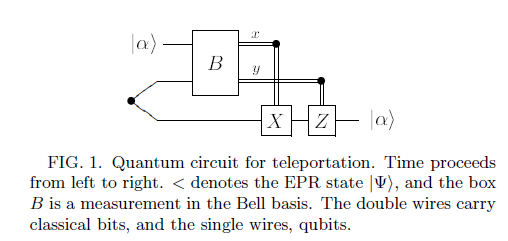
\includegraphics[width=1.0\textwidth]{images/quantum-information/quantenteleportation_cnot_1.png}
    \caption{Zeitstrahl von links nach rechts. B = Bell-Zustand, X Y Z = Pauli Operatoren, \(\ket{\alpha}\) = Zustand des Sender-Qubits, der an den Empfänger-Qubit übertragen werden soll}
    \label{fig:meinbild}
\end{figure}
\newpage
\noindent Dieses Prinzip kann leicht modifiziert werden. Die modifizierte Variante erlaubt es, vier Qubits, wovon jeweils zwei verschränkt sind und sich in einem Bell-Zustand befinden, durchzulassen und anhand von Pauli-Matrix Operationen zu transformieren. Die zwei Bell-Zustand Paare sind vorerst getrennt. Eines beinhaltet den „target“ Qubit \(\ket{\alpha}\), das andere den „control“ Qubit \(\ket{\beta}\). Der „target“ Qubit wird gedreht, wenn der „control“ Qubit einen Wert von \(\ket{1}\) hat. Es stehen 4 Rechenoperationen (I, X, Y, Z) zur Verfügung. Welche Operationen auf die Qubits der Bell-Zustände angewendet werden, ist vom Zufall bestimmt. Was aus dem CNOT gate herauskommt, sind zwei Qubits \(\ket{out}\), welche die Quanteninformationen von \(\ket{\alpha}\) und \(\ket{\beta}\) enthalten, wobei \(\ket{out}\) = CNOT\(\ket{\beta}\)\(\ket{\alpha}\).\\
\begin{figure}[h!]
    \centering
    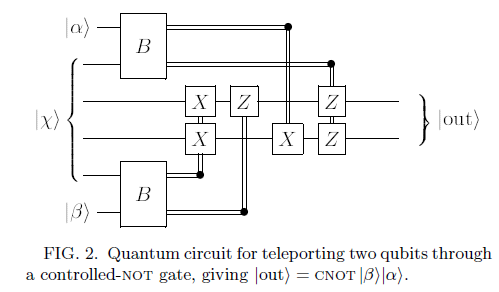
\includegraphics[width=1.0\textwidth]{images/quantum-information/quantenteleportation_cnot_2.png}
    \caption{Zeitstrahl von links nach rechts. B = Bell-Zustand, X Y Z = Pauli Operatoren, \(\ket{\chi}\) = Ausgangszustand für Operation}
    \label{fig:meinbild}
\end{figure}
\newpage
\noindent Eine andere modifizierte Variante ist eine, bei der ein CNOT gate zwischen zwei Qubits von zwei unterschiedlichen verschränkten Qubit Paaren geöffnet wird. Der Output von solch einem Gatter kann verwendet werden, um den Zustand \(\ket{\chi}\) der vorherigen Abbildung zu bilden, von dem in einer Quantenteleportation mit zwei Bell-Zuständen Gebrauch gemacht wird. \(\ket{\chi}\) kann so erzeugt werden, oder durch eine Quantenteleportation zwischen zwei GHZ (Greenberger Horne Zellinger) Zuständen. Ein GHZ Zustand ist eine Verschränkung von drei Quantenobjekten.\\
\begin{figure}[h!]
    \centering
    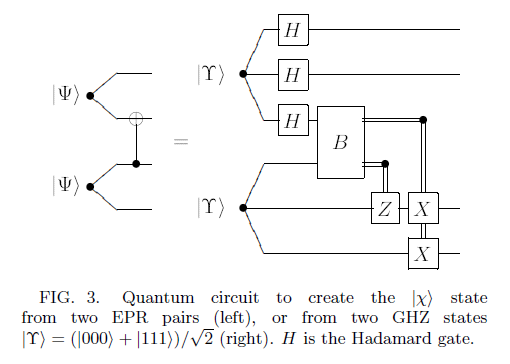
\includegraphics[width=1.0\textwidth]{images/quantum-information/quantenteleportation_cnot_3.png}
    \caption{Zeitstrahl von links nach rechts. \(\ket{\Upsilon}\) = GHZ Zustand, H = Hadamard gate (für Hadamard Transformation), B = Bell-Zustand, X Y Z = Pauli Operatoren}
    \label{fig:meinbild}
\end{figure}
\newpage

\subsection{Bedeutung für Quantenkommunikation und als Demonstration von Quanteninformationstransfer}
Wie Anhand der wissenschaftlichen Artikel von Bennett, Brassard et. al., sowie Gottesmann und Chuang gezeigt wurde, sind Quantenverschränkung und Quantenteleportation die Prinzipien, durch die es zu einem Quanteninformationstransfer kommen kann. Daraus kann man schließen, dass beide Prinzipien eine sehr wichtige Bedeutung für Quantenkommunikation haben.

\section{Bell-Zustand und Quantenkorrelation}

Um die theoretischen Grundlagen der Quanteninformation greifbarer zu machen, bietet sich der Bell-Zustand als anschauliches Beispiel an. Er veranschaulicht zentrale Konzepte wie Quantenverschränkung und Nichtlokalität und bildet die Grundlage für viele Anwendungen in der Quantenkommunikation und -verarbeitung. Im Folgenden wird der Bell-Zustand näher erläutert, seine mathematische Darstellung vorgestellt und seine Bedeutung anhand konkreter Experimente und Anwendungen verdeutlich

\subsection{Was ist ein Bell-Zustand?}
Bell-Zustände sind spezielle Zustände in der Quantenmechanik, in denen zwei Teilchen maximal miteinander verschränkt sind. Das bedeutet: Ihre Zustände hängen so stark zusammen, dass man sie nicht unabhängig voneinander beschreiben kann – selbst, wenn die Teilchen physisch weit voneinander entfernt sind. Benannt ist der Bell-Zustand nach dem Physiker John S. Bell. Dieser zeigte im Jahre 1964 auf, dass die Vorhersagen der Quantenmechanik im Widerspruch zu den Prinzipien des lokalen Realismus stehen – also der Vorstellung, dass Informationen nicht schneller als Licht übertragen werden können und physikalische Größen vor der Messung bereits festgelegt sind. (Vgl. \cite[S.195]{bell_einstein_1964})
\\


Mit der von John S. Bell formulierten Bell-Ungleichung entwickelte Bell ein mathematisches Kriterium, mit dem sich klassische und quantenmechanische Theorien experimentell unterscheiden lassen. Die Quantenmechanik sagt unter bestimmten Bedingungen eine Verletzung der nach John S. Bell benannten Bell-Ungleichung voraus. Belegt wurde dies in zahlreichen Experimenten ab 1972, den sogenannten Bell-Test. Seitdem wurde die Verletzung der Bell-Ungleichung in zahlreichen Experimenten mit verschränkten Teilchenpaaren eindeutig nachgewiesen. In allen Fällen bestätigten die Ergebnisse die Vorhersagen der Quantenmechanik. 
(Vgl. \cite[S.53-59]{homeister_quantum_2022})

\subsection{Die vier Bell-Zustände}
Insgesamt existieren vier verschiedene Bell-Zustände, die eine Situation maximaler Verschränkung zwischen zwei Qubits beschreiben. Das heißt: Wird der Zustand eines Qubits gemessen, ist das Ergebnis des anderen automatisch bestimmt. Unabhängig von der Entfernung der Qubits voneinander. (Vgl. \cite[S.53-55]{homeister_quantum_2022}) 
\\


Die vier Bell-Zustände sind nachfolgend dargestellt: 
\[
\begin{aligned}
\ket{\Phi^+} &= \frac{1}{\sqrt{2}} (\ket{00} + \ket{11}), \\
\ket{\Phi^-} &= \frac{1}{\sqrt{2}} (\ket{00} - \ket{11}), \\
\ket{\Psi^+} &= \frac{1}{\sqrt{2}} (\ket{01} + \ket{10}), \\
\ket{\Psi^-} &= \frac{1}{\sqrt{2}} (\ket{01} - \ket{10}).
\end{aligned}
\]

\subsection{Erzeugung eines Bell-Zustands}
Die Erzeugung eines Bell-Zustands basiert auf zwei Schritten. Zu Beginn wird eine Superposition erzeugt, anschließend muss die Verschränkung zwischen den Qubits hergestellt werden. Diese Schritte werden nachfolgend erläutert.
\\


\textbf{Schritt 1 – Superposition erzeugen:} \\
Zuerst wird auf das erste Qubit ein Hadamard-Gatter angewendet. Dadurch wird dieses Qubit in eine Superposition überführt:

\[
\frac{1}{\sqrt{2}} (\ket{0} + \ket{1}) \ket{0} = \frac{1}{\sqrt{2}} (\ket{00} + \ket{10})
\]
\\


\textbf{Schritt 2 – Verschränkung herstellen:} \\
Anschließend folgt ein CNOT-Gatter, bei dem das erste Qubit als Kontroll- und das zweite als Zielqubit fungiert. Dieses Gatter invertiert das Zielqubit nur dann, wenn das Kontrollqubit den Zustand \(\ket{1}\) hat. Dadurch entsteht der Zustand:

\[
\frac{1}{\sqrt{2}} (\ket{00} + \ket{11}) = \ket{\Phi^+}
\]
\\


Es resultiert die vollständige Quantenschaltung zur Erzeugung des Bell-Zustands. Diese ermöglicht es, jeden einfachen Zwei-Qubit-Eingangszustand (\(\ket{00}, \ket{01}, \ket{10}, \ket{11}\)) in einen Bell-Zustand zu überführen.

\begin{figure}[h]
  \centering
  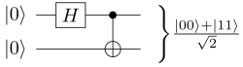
\includegraphics[width=0.5\textwidth]{images/quantum-information/bell_circuit.png}
  \caption{Quantenschaltung zur Erzeugung des Bell-Zustands}
\end{figure}


Es resultiert einer der zuvor vorgestellten Bell-Zustände – ein maximal verschränkter Zustand, in dem die Messungen der beiden Qubits perfekt korreliert sind. Wird in einem verschränkten Bell-Zustand das erste Qubit gemessen, so ergibt sich mit gleicher Wahrscheinlichkeit entweder der Zustand \( \ket{0} \) oder \( \ket{1} \). In beiden Fällen legt diese erste Messung sofort auch den Zustand des zweiten Qubits fest: Beobachtet man \( \ket{0} \) am ersten Qubit, ergibt sich insgesamt der Zustand \( \ket{00} \); misst man \( \ket{1} \), resultiert der Zustand \( \ket{11} \). Eine anschließende Messung des zweiten Qubits führt daher zwangsläufig zum gleichen Ergebnis wie beim ersten – entweder beide Qubits liefern 0 oder beide liefern 1. Je nach Eingangs-Zustand und der Reihenfolge der Gatter ergibt sich ein anderer Bell-Zustand. (Vgl. \cite[S.53-54]{homeister_quantum_2022})
\\


Ein anschauliches Beispiel für die Eigenschaften verschränkter Zustände liefert auch ein Gedankenexperiment mit zwei beispielhaften Personen, Alice und Bob. Angenommen die beiden erzeugten gemeinsam entsprechend der vorhergehenden Ausführungen folgenden Bell-Zustand:
\[
\frac{1}{\sqrt{2}} (|00\rangle + |11\rangle)
\]
Alice erhält nun das erste Qubit, Bob das zweite Qubit. Angenommen die beiden befinden sich, wie nachfolgend abgebildet, ursprünglich in einem Haus in verschiedenen Räumen. 

\begin{figure}[h]
  \centering
  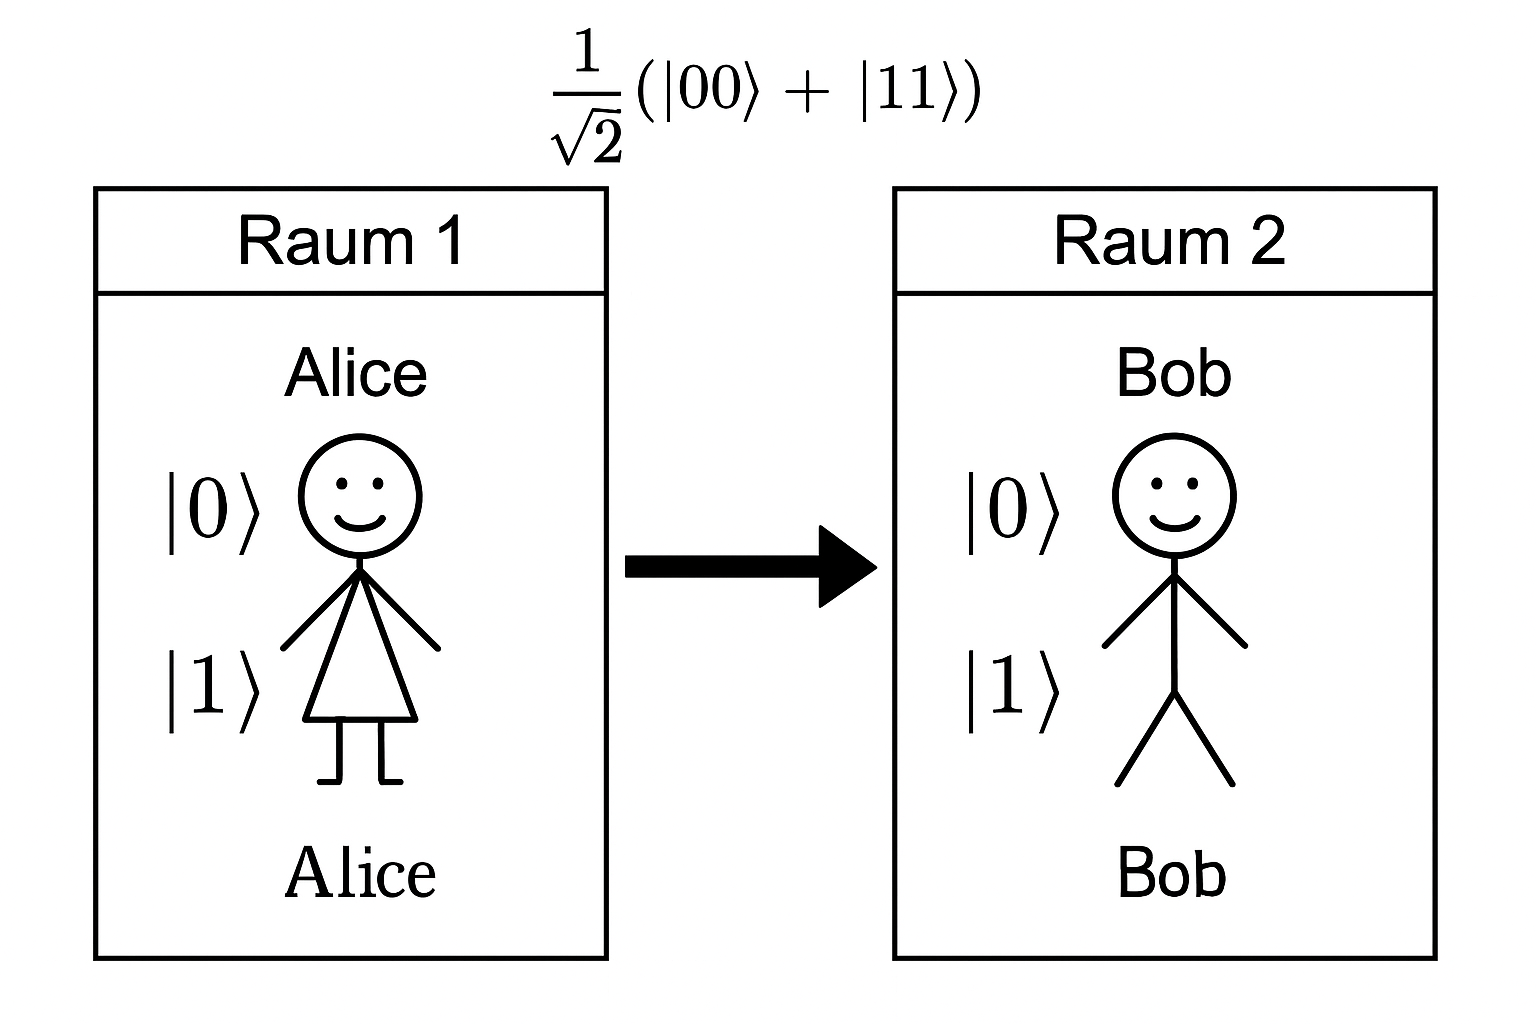
\includegraphics[width=0.5\textwidth]{images/quantum-information/Bell_Alice_Bob.png}
  \caption{Bell-Zustand: Alice und Bob}
\end{figure}


Solange nun keine Messung erfolgt und die Qubits vor äußeren Einflüssen geschützt sind, bleibt die Verschränkung erhalten – unabhängig von der räumlichen Trennung. Führen Alice oder Bob eine Messung durch, so ist das Ergebnis zufällig: Mit einer Wahrscheinlichkeit von 50\,\% wird $|0\rangle$ gemessen, mit 50\,\% $|1\rangle$. Erst wenn Alice und Bob ihre Ergebnisse miteinander vergleichen, zeigt sich die Besonderheit: Ihre Messergebnisse stimmen stets überein. Es resultiert eine perfekte Korrelation, unabhängig von Raum und Zeit. (Vgl. \cite[S.54]{homeister_quantum_2022})
\\


Genau darin zeigt sich der Informationsgehalt eines verschränkten Zustands: Die Information liegt nicht in einem einzelnen Qubit, sondern nur in ihrer gemeinsamen Beziehung. Diese Simulation macht das abstrakte Konzept der Quantenverschränkung greifbar und bietet einen intuitiven Zugang zu den Grundlagen der Quanteninformation. Es zeigt anschaulich, wie Quantencomputer fundamentale Prinzipien der Quantenmechanik sichtbar und messbar machen. 

\subsection{Bell-Zustand in der Praxis}

Bell-Zustände bilden das Fundament für viele Anwendungsfälle. Ein praktischer Anwendungsfall ist die Quantenkryptographie. Besonders bekannt ist insbesondere das sogenannte E91-Protokoll, welches auf dem Konzept der Quantenverschränkung beruht. Dabei erzeugt eine zentrale Quelle verschränkte Teilchenpaare und schickt je eines an zwei weit entfernte Personen – wie in unserem Beispiel etwa Alice und Bob. Wenn beide ihre Teilchen messen, erhalten sie stets perfekt korrelierte Ergebnisse. Dieser Effekt lässt sich nutzen, um einen gemeinsamen geheimen Schlüssel zu erzeugen. Ein Abhörversuch durch eine dritte Person würde diese Korrelation stören und könnte über einen Bell-Test erkannt werden. So kann mit Hilfe der Quantenmechanik sichergestellt werden, dass keine unbemerkte Informationsweitergabe stattgefunden hat – eine Grundlage für absolut sichere Kommunikation. (Vgl. \cite[S. 3841 f.]{kumar_state---art_2021})
\\


Quantenbasierte Protokolle stehen daher im Zentrum aktueller Forschung zur Quantenkryptographie und wurden bereits in ersten praktischen Experimenten erprobt. Besonders eindrucksvoll ist das Experiment mit dem chinesischen Micius-Satelliten: Er übermittelte verschränkte Photon-Bell-Paare an zwei Bodenstationen, die über eine Entfernung von rund 1200 Kilometern verteilt waren. Die gemessenen Korrelationen verletzten dabei deutlich die Bell-Ungleichung – ein klares Zeichen dafür, dass die beobachteten Effekte nicht durch klassische Physik erklärbar sind, sondern echte Quantenverschränkung vorliegt. Auf dieser Grundlage könnten über Kontinente hinweg geheime Schlüssel erzeugt und die Kommunikation verschlüsselt werden. (Vgl. \cite{ivezic_entanglement_2022})
\\


Ein zweiter praktischer Anwendungsfall des Bell-Zustands findet sich im Quantencomputing, genauer gesagt in der sogenannten Quantenteleportation. Dabei wird der Zustand eines Quantenbits (Qubit) von einem Ort zu einem anderen übertragen, ohne dass das Teilchen selbst physisch bewegt wird. Grundlage hierfür ist ein gemeinsam genutzter Bell-Zustand zwischen Sender (Alice) und Empfänger (Bob), der die nötige Verschränkung bereitstellt. Durch eine spezielle Messung auf Seiten von Alice und die Übermittlung zweier klassischer Bits kann Bob den ursprünglichen Zustand lokal wiederherstellen. (Vgl. \cite{bennett_teleporting_1993})
\\


Im Gegensatz zur Quantenkryptographie, bei der Sicherheit im Vordergrund steht, dient die Quanten-Teleportation der fehlerfreien Übertragung von Quanteninformation. Dies ist eine essenzielle Voraussetzung für die Vernetzung räumlich verteilter Quantencomputer. Sie gilt daher als Schlüsselfunktion zukünftiger Quantencomputer-Netzwerke, etwa im Rahmen eines „Quanteninternets“. (Vgl. \cite{ivezic_entanglement_2022}) Erste praktische Umsetzungen konnten dies bereits demonstrieren: 2017 gelang es ein Qubit über 1.400 km mit dem zuvor bereits erwähnten Satellit Micius erfolgreich zu teleportieren. (Vgl. \cite{ren_ground--satellite_2017})


\subsection{Simulation mit IBM Quantencomputer}
Die Eigenschaften von Bell-Zuständen lassen sich mithilfe von Quantencomputern, wie denen von IBM, direkt auf Hardware simulieren und beobachten. In diesem Beispiel wird ein einfacher Quantenschaltkreis in der IBM Quantum Learning Platform, gemäß der zuvor erläuterten Schritte zur Erzeugung eines Bell-Zustands, aufgebaut. Ausgangszustand sind zwei Qubits, die beide den Wert 0 haben. Zunächst wird auf das erste Qubit ein Hadamard-Gatter (rotes Gatter) angewendet. Dadurch ging es in eine Überlagerung aus „0“ und „1“ über. Anschließend folgt ein CNOT-Gatter (blaues Gatter), das die beiden Qubits miteinander verschränkt: Wenn das erste Qubit nun auf „1“ übergeht, kippt das zweite automatisch ebenfalls auf „1“. Das Ergebnis ist ein Zustand, in dem die Qubits perfekt miteinander verbunden sind – man spricht von einem verschränkten Zustand. 

\begin{figure}[h]
    \centering
    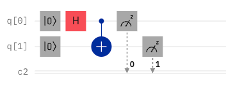
\includegraphics[width=0.6\textwidth]{images/quantum-information/Schaltung_IBM.png}
    \caption{Quantenschaltung - IBM Quantum Learning Platform.}
    \label{fig:meinbild}
\end{figure}

Nach dem Aufbau der Schaltung können über die IBM Quantum Learning Platform Messungen durchgeführt. Das bedeutet, dass die Qubits im Z-Basiszustand ausgelesen werden um zu überprüfen, ob sie im Zustand „0“ oder „1“ sind. 

\begin{figure}[ht]
    \centering
    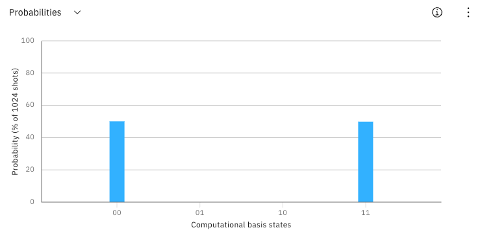
\includegraphics[width=1\textwidth]{images/quantum-information/results_ibm.png}
    \caption{Wahrscheinlichkeitsverteilung - IBM Quantum Learning Platform.}
    \label{fig:meinbild}
\end{figure}


Wie das Histogramm zeigt, werden ausschließlich die Zustände „00“ und „11“ beobachtet - und zwar mit jeweils rund 50\% Wahrscheinlichkeit. Die Zustände „01“ oder „10“, bei denen sich die beiden Qubits unterscheiden würden, treten gar nicht auf. Dies ist ein typisches Verhalten eines Bell-Zustands und belegt, dass die Qubits verschränkt sind. Bemerkenswert ist dabei: Diese Quantenkorrelation bleibt bestehen, selbst wenn die Qubits räumlich voneinander getrennt wären. Die Messergebnisse des einen beeinflussen scheinbar sofort das andere – ein Verhalten, das mit klassischer Physik nicht erklärbar ist. (Vgl. \cite{noauthor_bell_nodate}) 

\section{Zusammenfassung}
Dieses Kapitel hat gezeigt, dass Quanteninformation weit über das hinausgeht, was klassische Informatikmodelle leisten können. Durch die Einführung des Qubits als Informationsträger wurde deutlich, wie Superposition und Verschränkung völlig neue Rechenparadigmen ermöglichen. Die behandelten Quanten-Gatter, insbesondere die Pauli- und Hadamard-Gatter, bilden die Grundlage für alle quantenlogischen Operationen und Algorithmen. Mit den Beispielen des Deutsch- und Deutsch-Josza-Algorithmus wurde verdeutlicht, dass Quantencomputer bestimmte Probleme wesentlich effizienter lösen können als klassische Rechner. Außerdem wurde die Quantenverschränkung nicht nur als theoretisches Phänomen, sondern auch als praktisches Werkzeug für Teleportation, Kommunikation und Kryptographie vorgestellt. Die Bell-Zustände illustrierten dabei, wie stark verschränkte Systeme als Basis für sichere Kommunikation und Quantencomputing genutzt werden. Insgesamt bietet dieses Kapitel eine Grundlage, um die Funktionsweise und das Potenzial von Quantencomputern zu verstehen und bereitet darauf vor, in den kommenden Kapiteln tiefer in Hardware, Software und konkrete Anwendungen einzutauchen.

\printbibliography
